
% ===
\section{Significance of the Study}
% ===

This section outlines the significance of the study by presenting the expected results, a conceptual preview of the proposed framework, and the theoretical and practical implications of adopting an economic commensalism perspective. It also highlights potential avenues for future research and acknowledges possible limitations of the approach.

% ---
\subsection{Expected Results}
% ---

This research expects to demonstrate that endogenizing the environment as an active factor of production enables a more accurate identification of rational strategies that reconcile economic efficiency with ecological preservation. By integrating environmental feedbacks, marginal trade-offs, and intertemporal dynamics into production theory, the study aims to evaluate not only the volume of output, but the ecological consequences of the production process itself — that is, how it is produced, with what intensity of resource use, and at what environmental cost.

In particular, the proposed models seek to assess whether alternative configurations of the production-environment relationship — especially those based on commensal interactions — can achieve higher or more stable levels of output with lower marginal degradation. Using empirical data from the state of Mato Grosso, a region marked by both high productive potential and acute ecological pressure, the study will test whether the commensalism framework leads to sustainable and incentive-compatible equilibria in real-world territorial contexts.

% ---
\subsection{Conceptual Preview}
% ---

This study builds on the premise that conventional economics models — and the economy itself —, such as the standard Cobb-Douglas function, systematically exclude environmental variables or treat them as static constraints rather than productive factors. This limitation is particularly problematic in regions like the state of Mato Grosso, where high agricultural productivity intersects with sensitive biomes under increasing environmental pressure. The ecological stakes and economic incentives in such contexts demand a more integrated and dynamic representation of the production-environment relationship.

To address this, the thesis introduces the concept of economic commensalism, linking it to the central hypotheses and objectives formulated in the Research Design. Chapter 1 provides the ontological and epistemological justification for endogenizing environmental variables. Chapter 2 develops a formal model to test whether, under bounded rationality and incentive-compatible conditions, producers can achieve stable equilibria where preservation is individually rational. Chapter 3 empirically evaluates these dynamics in the case of Mato Grosso, testing whether areas under higher environmental integrity also exhibit higher marginal returns or reduced volatility in output.

To formalize this hypothesis, we consider a modified production function in which the environment ($E$) is treated as an endogenous and dynamic factor, alongside capital ($K$) and labor ($L$):

\[
Y = F(K, L, E)
\]

Under a commensalist configuration, the environment is not merely a passive input, but a regenerative factor that interacts with capital and labor in ways that can increase marginal productivity. This implies the following expected relationships:

\[
\frac{\partial Y}{\partial E} > 0, \quad 
\frac{\partial^2 Y}{\partial E^2} < 0, \quad
\frac{\partial^2 Y}{\partial K \partial E} > 0, \quad
\frac{\partial^2 Y}{\partial L \partial E} > 0
\]

\vspace{1em}

These conditions indicate that environmental input contributes positively to output (first derivative), but with diminishing returns (second derivative), and that the marginal productivity of capital and labor improves when the environment is preserved or enhanced — capturing the interdependence between natural systems and productive structures.

\vspace{1em}

This theoretical logic motivates the formal definition of the \textit{commensal advantage} ($\mathcal{C}$), representing the net production gain achieved by a commensalist strategy relative to an extractivist one, within the range where ecological integrity is still maintained:

\[
\mathcal{C} = 
\int_{x'}^{x^*} \left[ P_c(x) - P_e(x) \right] dx, 
\quad \text{where} \quad 
\begin{cases}
P_c(x) < x & \text{(ecological credit zone)} \\
P_e(x) > x & \text{(ecological debt zone)} \\
x^* < \bar{x} & \text{(before ecological collapse)}
\end{cases}
\]

Here, $P_c(x)$ and $P_e(x)$ denote the production levels under the commensalist and extractivist strategies, respectively, for a given level of environmental impact $x$. The integral $\mathcal{C}$ accumulates the marginal advantage of the commensalist configuration over the extractivist one between the arbitrary reference point $x'$ and the normative ecological bound $x^*$, which corresponds to the collapse of the mutualist trajectory, the most ecologically cautious yet economically limited strategy.

The vertical marker at $x^*$ defines the upper limit of the domain within which the commensalist model maintains normative legitimacy: beyond it, any further output would require crossing ecological thresholds or tolerating economic inefficiencies. The threshold $\bar{x}$ represents the collapse point of the predatory trajectory, beyond which no productive configuration remains ecologically sustainable.

However, a critical point in the diagram, denoted as $x_0$, marks the exact intersection between the predatory curve $P_{\text{pred}}(x)$ and the ecological balance line $X = Y$. This is referred to as the \textit{Predatory Equilibrium Threshold}. It represents the maximum level of environmental exploitation that the predatory strategy can sustain while still delivering economic output equal to or greater than its ecological cost. The coordinate of this point $(x_0, y_0)$ satisfies:

\[
P_{\text{pred}}(x_0) = x_0
\]

The shaded area between the predatory trajectory and the ecological balance line, from the origin to $x_0$, represents the \textit{ecological credit stock}, the total natural capital that can be extracted under a purely predatory regime without incurring ecological deficit. Beyond this point, the system generates environmental debt and enters a state of progressive degradation.

\vspace{1em}

\begin{figure}[H]
  \centering
  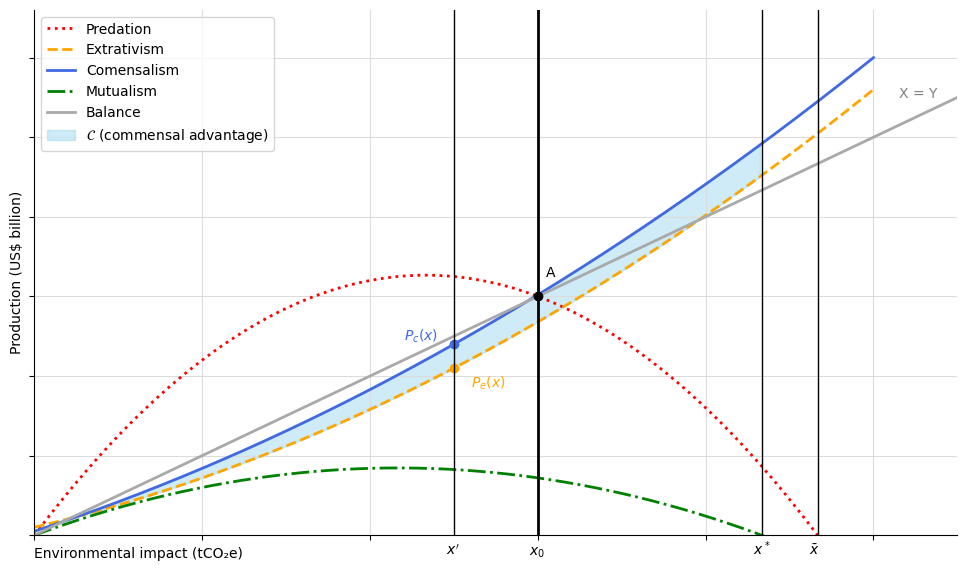
\includegraphics[width=\linewidth]{Figuras/eco_interactions.png}
  \vspace{-0.8em}
  \caption*{\textbf{\small Graph 1 – Theoretical supply curves under different ecological-economic strategies.}}
  \vspace{-0.5em}
  \caption*{\footnotesize Source: Author.}
  \label{graph1}
\end{figure}

Graph 1 compares the four ecological-economic paradigms examined in this research, which will be formally conceptualized in Chapter 1, by plotting production ($Y$, in US\$ billion) against environmental impact ($X$, in tons of CO\textsubscript{2}). The gray diagonal line ($X = Y$) represents a sustainability threshold: points above this line indicate that environmental costs exceed economic returns (ecological inefficiency), while points below suggest that production remains ecologically efficient relative to its footprint.

The \textit{predatory curve} (red, dotted) illustrates this dynamic most dramatically. It rises sharply as natural resources are exploited rapidly, but soon reaches a peak and collapses. This trajectory reflects the classical \textit{tragedy of the commons}: short-term maximization leads to irreversible ecological degradation and long-term economic failure. The critical intersection between the predatory trajectory and the balance line, labeled as point $A$ in the graph, is referred to as the \textit{Predatory Equilibrium Threshold} ($x_0$). It marks the end of the ecological credit zone for unsustainable models and represents the boundary of permissible exploitation under high-impact dynamics.

From the perspective of economic commensalism, the shaded area beneath the predatory curve and above the ecological equilibrium line ($X = Y$), from the origin up to $x_0$, can be interpreted as the total ecological stock that a biome or territory can endure before entering irreversible decline. Beyond this point, the system enters a state of net ecological debt, making even high-output strategies economically and ecologically unjustifiable.

The \textit{extractivist curve} (orange, dashed) attempts to moderate this collapse through legal or institutional constraints. While it temporarily extends the productive lifespan of the system, it eventually surpasses the sustainability threshold, indicating that even regulated extraction becomes ecologically inefficient over time. The model fails to maximize long-term productivity and does not prevent cumulative environmental degradation.

The \textit{mutualist curve} (green, dash-dotted) represents a normative ideal found in many conservation policies. It is modeled here as a concave quadratic function with low elasticity, capturing a regime of cautious use and diminishing marginal returns. It remains entirely below the balance line, reflecting ecological prudence, but reaches only modest productivity levels. Such strategies may preserve ecological integrity but tend to be economically unviable without ongoing subsidies or strong non-market incentives.

In contrast, the \textit{commensalist curve} (blue, solid), central to this research, begins conservatively but eventually surpasses the extractivist model in productivity, while remaining closer to the sustainability threshold throughout. Its long-run advantage lies not in avoiding environmental impact entirely, but in producing greater economic returns per unit of ecological cost. This reflects a strategic use of the environment as a regenerative and intertemporal factor of production, rather than a passive input to be depleted.

In this configuration, the difference between the commensalist and extractivist curves, when calculated separately in the regions above and below the balance line, defines the \textit{commensal advantage}: a net gain in production achieved with proportionally lower ecological burden. Chapter 2 will formally assess whether this differential is provable through dynamic optimization, under uncertainty, learning, and adaptive behavior.

Graph 1 also highlights the conceptual role of the integral $\mathcal{C}$, as well as the analytical relevance of the thresholds $x^*$ (end of economic viability of the mutualist model), $\bar{x}$ (collapse of the predatory model), and $x_0$ (ecological equilibrium breach under predation). These landmarks delimit the theoretical scope within which this research aims to demonstrate that a properly incentivized commensal strategy can outperform extractivist alternatives both economically and ecologically. This framework lays the foundation for the simulations developed in Chapter 2.

Integrating ecological categories such as commensalism, mutualism, and predation into economic reasoning helps to overcome the limitations of the current extractivist paradigm, which treats nature merely as a stock of resources to be exploited. Doing so enables a more refined understanding of how ecological dynamics influence production, resilience, long-term sustainability, and allows us to theorize environmental preservation not as a moral constraint, but as a rational economic strategy.

In this context, commensalism is proposed as a conceptual and analytical lens through which to model the asymmetric relationship between productive agents and the environment. Borrowed from ecology, the term denotes a form of interaction in which one party benefits while the other is neither harmed nor helped, a metaphor that, while symbolic, carries deep analytical weight. It suggests that the economy need not function as a parasite upon nature, but can instead coexist with it in a non-degradative and strategically beneficial manner, provided appropriate institutional and incentive structures are in place. 

% ---
\subsection{Implications}
% ---

This study holds the potential to generate both theoretical and practical implications by bridging economics and ecology through a rational, incentive-based framework. Conceptually, it contributes to rethinking production theory by integrating environmental dynamics as endogenous variables. Practically, it opens new pathways for policy design, business models, and institutional arrangements that align profitability with ecological resilience. In doing so, it creates space for socially inclusive and economically viable opportunities rooted in a more rational and productive use of natural resources.

%...
\subsubsection{Theoretical Contributions}
%...

This research presents an innovative framework for reconciling environmental conservation with economic efficiency. The proposed methodology, combining dynamic modeling, game theory, and econometric validation, offers a structured approach to designing market-compatible conservation policies. While ambitious, the model has the potential to inform both academic discourse and real-world policy applications.

This is evident when comparing the different theoretical understandings, preliminarily explained in the introductory topic, with the proposal of this work, to be verified and matured during the course of the research.

% INICIO TABELA 1
\renewcommand{\arraystretch}{1.3}

\begin{table}[H]
\centering
\caption{Comparative perspectives on the environment in economic and ecological theories}
\footnotesize % Tamanho da fonte
\resizebox{\textwidth}{!}{%
\begin{tabularx}{\textwidth}{lXXXXX}
\toprule
\textbf{Element} & \textbf{Classical-Neoclassical Economics} & \textbf{Institutional Economics} & \textbf{Ecology and Philosophy} & \textbf{Green Economy} & \textbf{Economic Commensalism (proposed)} \\
\midrule

\textbf{Land Factor} 
& Fixed production factor with diminishing returns; often absorbed into capital (\(K\)).
& Governed by property rights, access rules, and institutional power.
& Foundational and irreplaceable basis of life and ecological balance.
& Natural capital to be priced and incorporated into accounts.
& Dynamic ecological stock with productive potential and strategic reserve function. \\

\textbf{Environment} 
& Externality to be corrected via taxes or regulation.
& Common good subject to institutional failure  (Tragedy of the Commons). 
& Systemic interdependence. It has only intrinsic value. 
& Complementary asset with economic and ecological value. 
& Endogenous strategic factor; source of productivity and ecological payoff. \\

\textbf{Incentives logic} 
& Driven by prices and utility/profit maximization. 
& Shaped by rules, norms, and transaction costs.
& Ethics, ecological responsibility, and limits of growth.
& Financial and regulatory incentives for sustainability 
& Rational, territory-specific, dynamic incentives promoting cooperation and preservation. \\

\textbf{Time treatment} 
& Intertemporal optimization with fixed discounting.
& Path-dependent institutional evolution over time.
& Quasi-irreversible ecological processes.
& Inter-generational planning and ecological risk management.
& Strategic long-term rationality; preservation as anticipatory production logic. \\

\textbf{Unit of analysis} 
& Rational agent (homo economicus).
& Groups, communities, and institutional arrangements. 
& Ecological systems, species interactions, biotic communities. 
& Population and territory with environmental footprint. 
& Rational agent interacting with environment and others under ecological constraints. \\

\textbf{Normative goal} 
& Allocative efficiency and competitive equilibrium 
& Institutional stability and minimization of governance failures. 
& Balance between society and nature; ecological integrity. 
& Economic, ecological, and social sustainability. 
& Alignment of economic rationality with environmental resilience and collective benefit. \\

\bottomrule
\end{tabularx}}

\vspace{0.1em}
\begin{flushleft}
\footnotesize
\textbf{Source:} Author, based on cited literature.
\end{flushleft}

\end{table}
% FIM TABELA 1

In this regard, it is important to emphasize that, given the motivations, hypotheses and purposes of this work, it is necessary to define that the term commensalism is not presented here as an aesthetic analogy, but aims to establish an institutional model of incentives, with implications for public policies, legal design and game theory. To this end, according to the methodology presented, the issue must be investigated in more depth and the hypotheses tested.

%...
\subsubsection{Practical Contributions}
%...

In practical terms, economic commensalism proposes an institutional shift in how environmental variables are treated within productive systems. Rather than framing preservation as a constraint or as a moral obligation, this approach treats environmental integrity as a productive asset that generates returns when preserved and signals ecological costs when degraded. This reconfiguration creates the basis for measurable ecological accountability, incentive-compatible preservation contracts, and financial innovations rooted in real, localized ecological data.

The comparative evidence across biomes, as shown in Table 2, reveals a critical dissonance between legal requirements and scientific tipping points. In the Amazon, where current legal protections exceed the scientific thresholds, preservation is relatively aligned with ecological resilience. However, in the Cerrado and Pantanal, legal baselines are dangerously below ecological thresholds, exposing these regions to irreversible degradation. A commensalist framework can help recalibrate these legal requirements using biophysical indicators, moving toward a dynamic and territory-specific model that anticipates ecological risk rather than reacting to its consequences.

% INICIO TABELA 2
\begin{table}[H]
\centering
\caption{Comparison between Deforestation, Scientific Tipping Points and Legal Requirements by Biome}
\label{tab:biomes_threshold}
\footnotesize
\renewcommand{\arraystretch}{1.3}
\begin{tabularx}{\textwidth}{|l|c|c|c|X|}
\hline
\textbf{Biome} & 
\textbf{\begin{tabular}[c]{@{}c@{}}Cumulative\\ Deforestation (\%)\end{tabular}} & 
\textbf{\begin{tabular}[c]{@{}c@{}}Scientific\\ Tipping Point (\%)\end{tabular}} & 
\textbf{\begin{tabular}[c]{@{}c@{}}Legal\\ Requirement (\%)\end{tabular}} & 
\textbf{Alignment with Science} \\ 
\hline

Amazon & 
\textasciitilde17\% & 
20-25\% & 
80\% & 
High (protection above critical threshold) \\ 
\hline

Cerrado & 
\textasciitilde50\% & 
45-55\% & 
20-35\% & 
Low (legal limit below ecological threshold) \\ 
\hline

Pantanal & 
\textasciitilde25\% & 
30\% (hydrological regime) & 
20\% & 
Very low (risk not considered) \\ 
\hline

\end{tabularx}

\vspace{0.1em}
\begin{flushleft}
\footnotesize
\textbf{Source:} Based on \citeonline{lenton2008tipping}, \citeonline{lovejoy2018amazon}, and \citeonline{IPCC2023}.
\end{flushleft}

\end{table}
% FIM TABELA 2

Carbon markets, currently underutilized or poorly regulated, especially at the subnational level, could be radically improved under a commensal logic. Instead of speculative mechanisms disconnected from ecological performance, local carbon pricing and compensation schemes would be anchored in actual biophysical integrity, incentivizing producers to maximize output within ecological safety zones. Instruments such as REDD+, green bonds, CRAs (Certificates of Agribusiness Receivables), and PRAs (Environmental Regularization Programs) would gain effectiveness by shifting from punitive compliance models to reward-based, performance-linked contracts.

In the case of Mato Grosso, where agricultural frontiers coincide with some of the world's most endangered ecosystems, economic commensalism could unlock a new generation of public policies. These would promote preservation not by imposing restrictions, but by enhancing the profitability of sustainable practices. Producers would be motivated to invest in advanced monitoring technologies (such as IoT-based land tracking, AI-enabled forecasting, or precision machinery), not only for productive efficiency but also for environmental certification, credit access, and territorial premiums. This dual payoff structure, productivity and preservation, would improve investment decisions, reduce long-term risk, and expand financial access for rural producers.

Ultimately, the commensalist framework suggests a paradigm shift: from fragmented environmental policy to integrated territorial governance; from reactive command-and-control instruments to proactive ecological valuation; and from short-term extraction to long-term strategic use of natural capital. These transformations carry not only environmental and economic benefits, but also open a path for inclusive development models that reconcile production with the safeguarding of critical ecosystems.

%...
\subsubsection{Research Opportunities}
%...

The approach introduced in this study represents an attempt to compel a major shift in how environmental variables are interpreted, valued, and integrated into economic systems, particularly in frontier areas such as Mato Grosso, where environmental pressures and productive growth are closely intertwined. By transcending a reactive and extractivist mindset, economic commensalism aims to redefine nature not as a mere limitation, but as a dynamic asset capable of providing economic returns. If this perspective proves viable and theoretically sound, the resulting ontological paradigm change will position ecological preservation as a source of revenue and intrinsic value, transforming forests, ecotones, and other preserved ecosystems into fixed capital and financial assets.

From a practical standpoint, this would imply a new architecture for environmental finance. Instead of viewing producers only through the lens of legal compliance, banks and credit institutions can assess their environmental stock — their preserved hectares — as a tangible component of creditworthiness. This will enable the integration of an environmental score into rural credit models and the structured issuance of green financial instruments such as green bonds, CRAs, and sustainability-linked loans indexed to ecological metrics. Under a commensalist logic, landowners would be incentivized to preserve biomes not by coercion, but because the opportunity cost of deforestation would exceed the long-term returns from maintaining ecosystem integrity, especially if local carbon pricing systems become more transparent and decentralized.

Unlike today’s “green” financial instruments, which often operate under a merely cosmetic logic, rewarding actors for not exceeding minimum thresholds, the commensalist framework invites a transition from compensation to value generation without degradation. It promotes investment in capital and labor (particularly human capital), while reducing pressure on natural assets like land and hydrological cycles. Moreover, if our theoretical proposal proves to be coherent, logically valid, and supported by real evidence that its assumptions work in the factual world, it will curb speculative or exaggerated claims from environmental asset sellers by tying remuneration to verifiable local performance, rather than to opaque offset structures. In doing so, it would enhance both the legitimacy and the efficiency of carbon markets and regulatory mechanisms.

Incidentally, in theoretical terms, the introduction of the concept of economic commensalism reorients economic thought itself: from marginalist models based on scarcity and substitution, to integrated systems where preservation and production are jointly optimized. By treating the environment as an endogenous and flexible input, subject to local thresholds and ecological tipping points, this framework allows for a more rational allocation of resources. It enables public policy to move from rigid command-and-control approaches to adaptive, incentive-compatible strategies that better reflect the diversity of biomes and socio-productive realities. In sum, the research opens new avenues for aligning private rationality with public sustainability goals, not by moral persuasion, but through a new institutional logic grounded in ecological productivity and economic profitability.

% ---
\subsection{Possibly Limitations}
% ---

As an emerging and exploratory framework, our research may encounter theoretical and formalization challenges, especially in aligning ecological concepts with established economic modeling tools. Translating ecological dynamics, such as resilience, tipping points, and asymmetrical dependence, into consistent mathematical and econometric models remains a demanding task that may require iterative refinement.

Empirically, the study may also face constraints related to the availability and reliability of disaggregated environmental data — particularly at the biome and property levels in Mato Grosso. Incomplete or outdated land use information, limited access to verified carbon data, and lack of standardized ecological indicators may restrict the precision of empirical tests. These limitations do not invalidate the research but call for cautious interpretation and future methodological adaptations.

\newpage

% fim %